\chapter{Proposta de extensão}\label{chp:extensao}

O projeto até o momento enfrentou diversos desafios e buscou desempenhar muitos testes até decidirmos escolher meio de começar a elaboração do \textit{VCranium} (Capítulo "\nameref{chp:criacao-vcranium}"). A pesquisa bibliográfica mostrou a possibilidade, por meio de diferentes técnicas, de aplicarmos o \textit{Moverio BT-350} no ambiente cirúrgico e, especialmente, na neurocirurgia \cite{Cho2020}. A extensão do período de trabalho no projeto, assim como a renovação da bolsa, trará também o aprofundamento e refinamento dos processos implementados no programa.

Com a arquitetura do sistema montada, temos um cenário propício para continuar a desenvolver atualizações que permitam uma melhor estabilidade e compatibilidade com os recursos dos óculos. Isto posto, podemos não só refinar o algoritmo atual de detecção por marcadores, como podemos aplicar redes treinadas de \textit{machine learning} ou utilizar o modelo da \textit{Intel RealSense} do laboratório para o uso de \textit{surface matching} da superfície da cabeça do paciente, ambas técnicas já sendo estudadas por outros pesquisadores do \textit{AeroTech}.

\begin{figure}[ht]
    \centering
    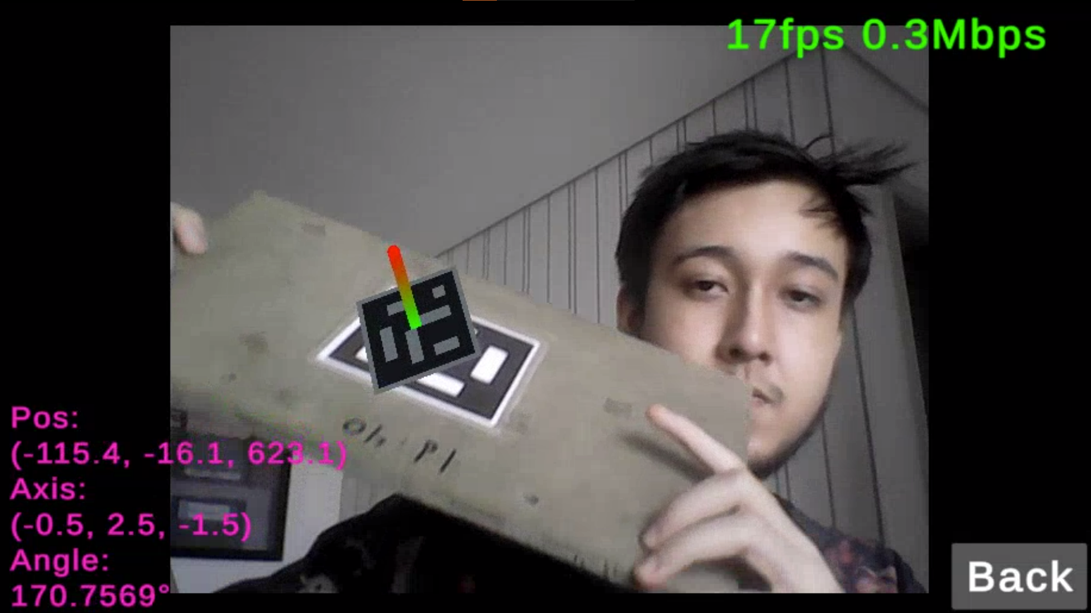
\includegraphics[width=.6\linewidth]{figuras/vcranium_calibration.png}
    \caption{Erro de projeção por falta de calibração da câmera. Fonte: Autor.}
    \label{fig:vcranium-calibration}
\end{figure}

O próximo passo do \textit{VCranium} é a calibração da projeção em realidade aumentada. Visto que a observação do usuário dos óculos é estereoscópica, a primeira parte de viabilizar a exibição de AR é fazer a visualização independente para cada olho. Para isso, é necessário um cálculo de calibração particular de cada usuário, e além disso, garantir que essa calibração se mantenha todas as transformações da projeção no espaço virtual. Atualmente, o projeto se encontra desregulado na projeção, não criando o efeito de sobreposição adequado (Figura \ref{fig:vcranium-calibration}).

\section{Objetivo}

Trabalhar na arquitetura de sistema montado no primeiro período da pesquisa, que envolverá os compromissos de refinar o método atual de estimação de posição por marcadores; experimentar diferentes métodos de visão computacional; e comparar com os dados de precisão da literatura. Dessa maneira, cooperando com o objetivo primordial de aumentar a proximidade do neurocirurgião com a tecnologia \textit{AR} em procedimentos cirúrgicos.  

\section{Metodologia}

Como trata-se de um projeto com um sistema já definido, a metodologia precisa dar ênfase no conhecimento da confiabilidade dos métodos. Por isso, consistirá no estudo matemático das projeções e as demonstrações das técnicas que colaboram com o objetivo da projeção AR e, por conseguinte, dissertações e apresentação dos resultados em tabelas também serão produzidos. Ainda que a metodologia terá destaque no aprofundamento dos métodos, as pesquisas de novos artigos serão feitas conjuntamente com esses estudos, procurando monitorar as descobertas e novos resultados no campo de realidade aumentada aplicada em cirurgias.

\newpage

\section{Cronograma}

O controle de atividades vai ser feito com encontros mensais e semanais com o coorientador, orientador e integrantes do laboratório. Um cronograma foi elaborado na tabela \ref{fig:tabela} para servir de guia para o progresso do projeto.

\begin{table}[h]
    \begin{tabular}{llllllll} 
        \hline
\multicolumn{8}{c}{\textbf{Cronograma de atividades para a extensão}} \\ 
\hline
& & & {\cellcolor[rgb]{.3,.3,1}} & \multicolumn{4}{l}{Execução} \\ 
    \hline
 \textbf{Atividade} & \textbf{Bimestre} & 1 & 2 & 3 & 4 & 5 & 6 \\ 
    \hline
 \begin{tabular}[c]{@{}>{}l@{}}Revisão e refinamento dos códigos do VCranium \\\end{tabular} & & {\cellcolor[rgb]{.3,.3,1}} & & & & & \\ 
    \hline
 Estudo sobre calibração de projeção AR & & {\cellcolor[rgb]{.3,.3,1}} & {\cellcolor[rgb]{.3,.3,1}} & & & & \\ 
    \hline
 Aprofundamento em calibração estereoscópica Moverio & & & {\cellcolor[rgb]{.3,.3,1}} & {\cellcolor[rgb]{.3,.3,1}} & & & \\ 
    \hline
 Testes com outros algoritmos de detecção & & & & & {\cellcolor[rgb]{.3,.3,1}} & {\cellcolor[rgb]{.3,.3,1}} & \\ 
    \hline
 Coleta de dados da precisão de métodos* & & & & & {\cellcolor[rgb]{.3,.3,1}} & {\cellcolor[rgb]{.3,.3,1}} & {\cellcolor[rgb]{.3,.3,1}}  \\
    \hline
    \end{tabular}
    \caption{*A coleta de dados pode envolver o auxílio da parceria do Centro de Cirurgia de Epilepsia (CIREP) do Hospital das Clínicas da Faculdade de Medicina de Ribeirão Preto-USP}
    \label{fig:tabela}
\end{table}